\begin{figure}[!h]
  \centering
  \begin{subfigure}{.4\textwidth}
    \centering
    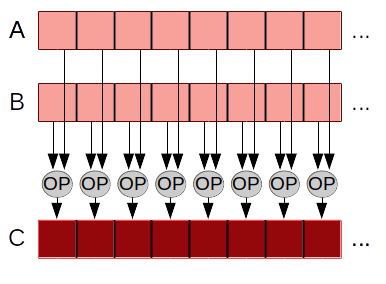
\includegraphics[width=\textwidth]{img/SIMD_scalar.png}
    \caption{Code scalaire}
    \label{fig:SIMD:scalar}
  \end{subfigure}
  \begin{subfigure}{.4\textwidth}
    \centering
    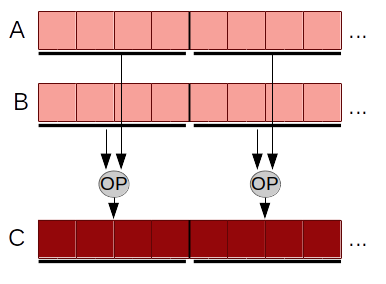
\includegraphics[width=\textwidth]{img/SIMD_vect.png}
    \caption{Code vectoriel}
    \label{fig:SIMD:vect}
  \end{subfigure}
  \caption{Illustration du fonctionnement des instructions SIMD pour un opérateur donné, appliqué à des éléments consécutifs. Dans la version scalaire (\ref{fig:SIMD:scalar}), l'opérateur est appliqué à chacun des éléments des tableaux A et B deux à deux. Si le processeur dispose d'instructions vectorielles, il est possible de charger simultanément plusieurs éléments consécutifs et de leur appliquer le même opérateur simultanément (\ref{fig:SIMD:vect}), permettant de réduire le nombre d'opérations à effectuer.}
  \label{fig:SIMD}
\end{figure}
